\chapter{03. IoT Architecture}

\section{IoT System Architecture}

\subsection{Communication Paradigms}
\begin{itemize}
    \item \textbf{Client/Server}: sources explicitly know the destination of their messages.
    \item \textbf{Publish/Subscribe}: sources publish to a logical channel; interested destinations subscribe (one-to-many, no explicit sessions).
    \item Typical IoT traffic flows:
    \begin{itemize}
        \item \textbf{Asynchronous events} (uplink)
        \item \textbf{Periodic or on-demand measurements} (uplink)
        \item \textbf{Commands} from processing platforms (downlink)
    \end{itemize}
\end{itemize}

\subsection{Properties of an IoT System}
\begin{itemize}
    \item \textbf{Trustworthiness}: availability, resilience, confidentiality, integrity, safety.
    \item \textbf{Architectural}: composability, modularity, heterogeneity, scalability, legacy support, shareability, unique identification.
    \item \textbf{Functional}: accuracy, auto-configuration, context-awareness, big data management, discoverability, real-time, self-description, compliance.
\end{itemize}

\subsection{Standard Reference Model}
\begin{itemize}
    \item \textbf{Physical Entity Domain (PED)}: monitored physical objects.
    \item \textbf{Sensing \& Controlling Domain (SCD)}: sensors, actuators bridging physical $\leftrightarrow$ cyber world.
    \item \textbf{Operations \& Management Domain (OMD)}: OSS + BSS for provisioning, assurance, optimization.
    \item \textbf{Resource Access \& Interchange Domain (RAID)}: service interfaces with access policies.
    \item \textbf{Application \& Service Domain (ASD)}: end-user services via APIs or portals.
    \item \textbf{User Domain (UD)}: human/digital users via devices (PCs, smartphones, control panels, smart glasses)
\end{itemize}

\begin{figure}[h]
    \centering
    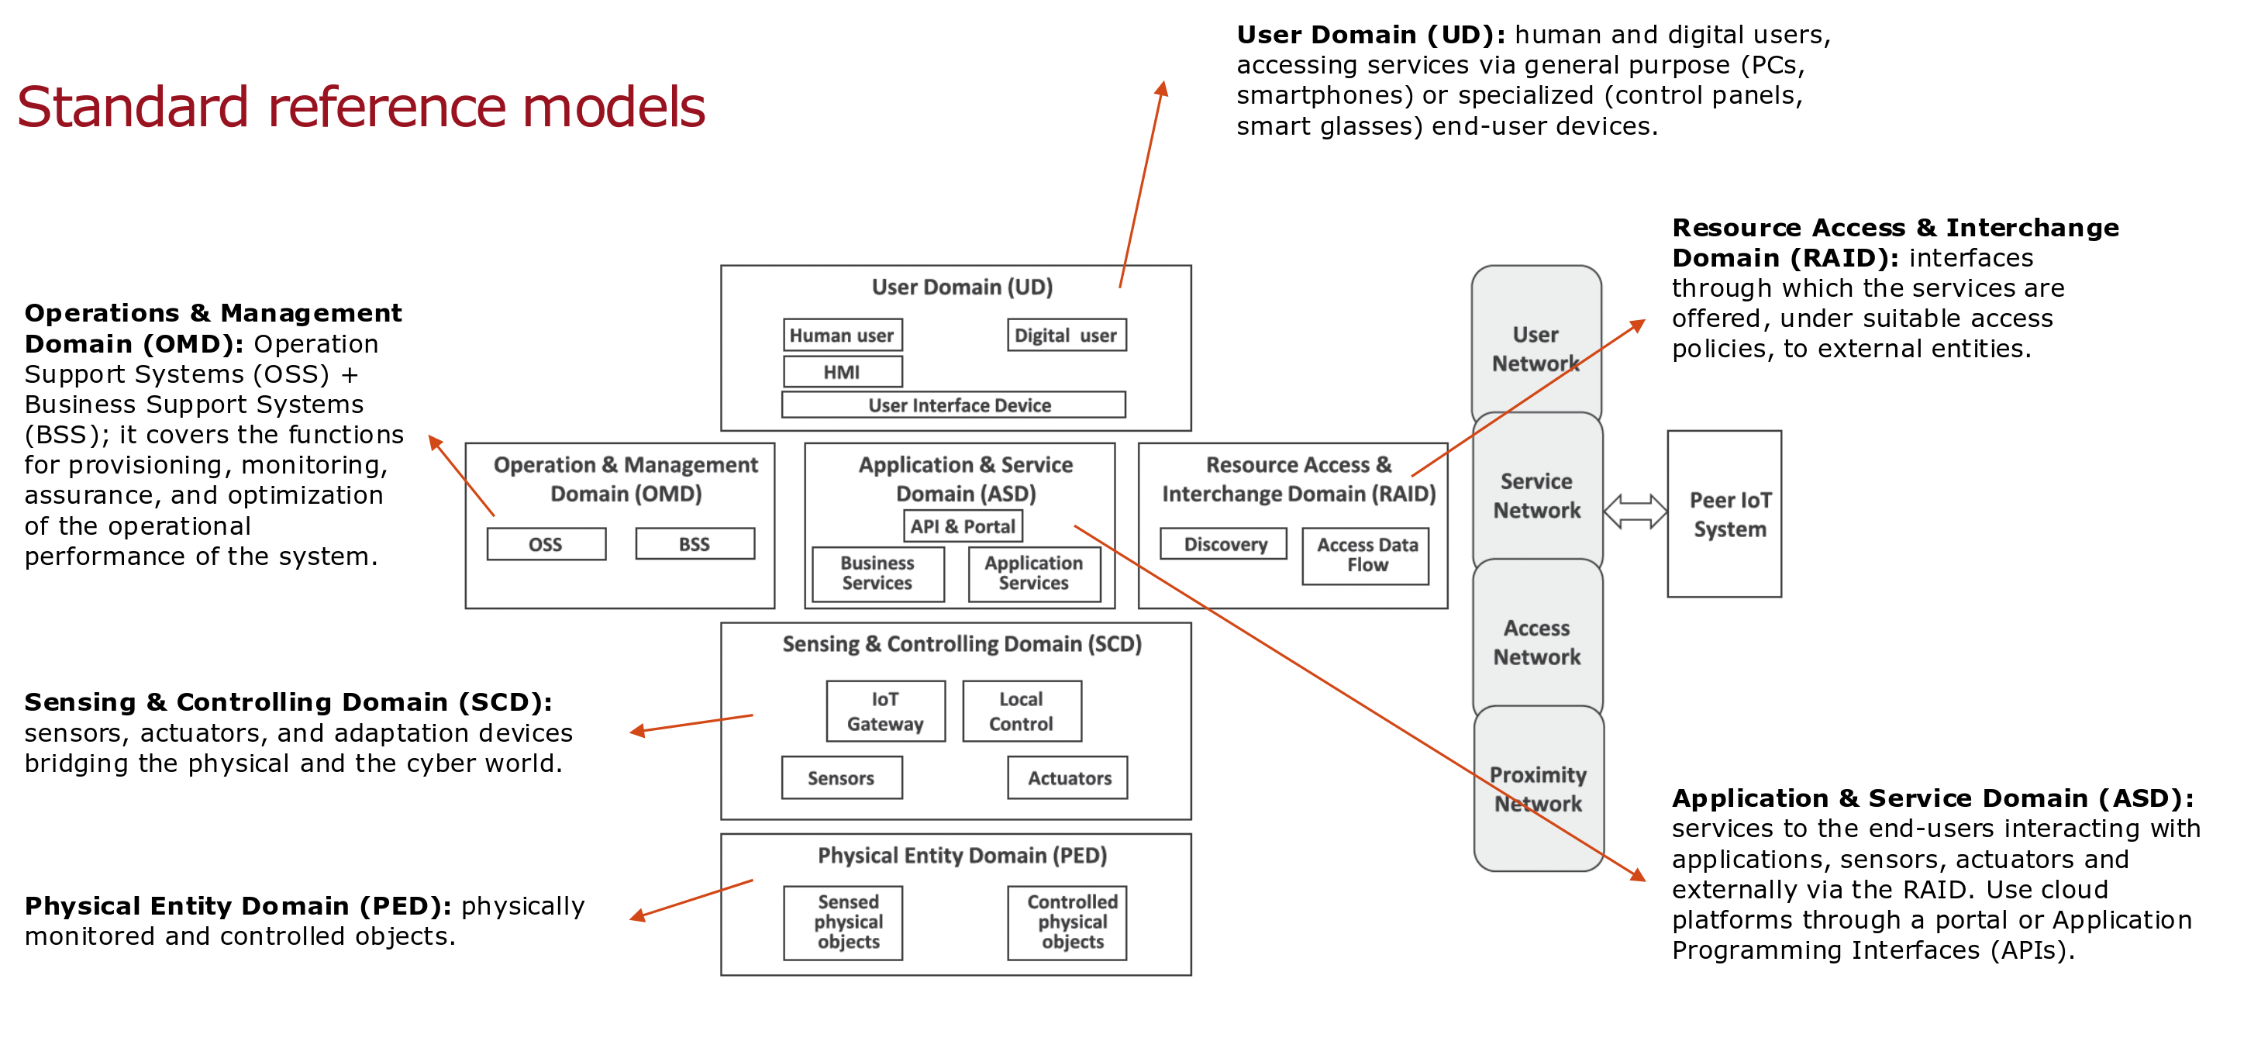
\includegraphics[width=0.8\textwidth]{Images/Pasted image 20251001094808.png}
    \caption{IoT Standard Reference Model}
\end{figure}

\subsection{Network Architectures}
\begin{itemize}
    \item \textbf{One-level}: endpoints use full IP stack (e.g., cellular).
    \item \textbf{Two-level (1b)}: endpoints resource-constrained, gateway manages protocols (LPWA, Low Power Wide Area: LoRa, SigFox, NB-IoT). \textit{Target of the course}
    \item \textbf{Two-level (1c)}: endpoints support TCP/IP, traffic managed by router (Ethernet/Wi-Fi)
\end{itemize}

\subsection{WANs}
\begin{itemize}
    \item TCP/IP networks, shared among users.
    \item Public by nature.
    \item \textbf{VPNs}: reserved bandwidth/security for defined groups, with private IP addressing
    \item Users outside of a group cannot communicate directly with users of the group.
    \item Use private IP addressing and private routing protocol instances.
\end{itemize}

\subsection{Topologies}
\begin{itemize}
    \item \textbf{Bus}: every nodes taps into a shared medium (CSMA/CD), collisions possible.
    \item \textbf{Ring}: token-based, eliminates collisions, requires token management.
    \item \textbf{Star}: master/slave, predictable, not scalable (master bottleneck).
    \item \textbf{Mesh}: full or partial, robust, private, many physical links
\end{itemize}

\section{Endpoints}

\subsection{Sensors}
\begin{itemize}
    \item Devices detecting stimuli $\rightarrow$ electrical/processable output.
    \item Types: pressure, temperature, biometric, chemical, acoustic, optical, positioning, etc.
    \item Three classifications:
    \begin{itemize}
        \item \textbf{Fixed}: stable, not moving like domotics
        \item \textbf{Mobile}: always moving (GPS, wearables)
        \item \textbf{Nomadic}: they move but then they stop somewhere else (portable medical devices, field sensors)
    \end{itemize}
    \item \textbf{Active vs Passive} sensors
    \begin{itemize}
        \item \textbf{Active}: need to run a current or send a signal to get a measurement (e.g., clocks, strain gauges, radar).
        \item \textbf{Passive}: use the physical phenomenon itself (e.g., piezoaccelerometers, GPS, thermocouples).
    \end{itemize}
\end{itemize}

\subsubsection{Actuators}
\begin{itemize}
    \item Output elements performing actions.
    \item \textbf{Digital}: on/off switching.
    \item \textbf{Analog}: continuous signals (e.g., motor speed control).
\end{itemize}

\subsubsection{Gateways}
\begin{itemize}
    \item Bridge sensors $\leftrightarrow$ higher-level processing/cloud.
    \item Provide connectivity, data collection, filtering, storage, event processing, optional analytics
\end{itemize}

\subsubsection{Fog Nodes}
\begin{itemize}
    \item ``Bring the cloud to the ground.''
    \item More powerful than gateways, allow \textbf{local analytics with lower latency}.
\end{itemize}

\section{Data plane functions}

\subsection{Data acquisition and processing}

In order to get a digital signal from a sensor, we need to account for:
\begin{itemize}
    \item Sampling
    \item Aliasing
    \item Quantization
    \item Saturation
    \item Hysteresis and non-linearities
    \item Calibration
    \item Error propagation
\end{itemize}

\subsubsection{Sampling}

\begin{itemize}
    \item First, we sample: we take (regular) measurements over time, and represent the signal with those measurements.
    \item Nyquist theorem: if sampling is $\geq$ twice as fast as the signal, sampling has no errors.
    \item Example: If a signal is thought to have a maximum frequency between 1000 Hz and 4000 Hz, which of the following would be the most appropriate sample rate?
    \begin{itemize}
        \item a. 500 Hz
        \item b. 8000 Hz
        \item c. 9000 Hz
        \item d. 24000 Hz
    \end{itemize}
\end{itemize}

\subsubsection{Aliasing}
\begin{itemize}
    \item If we do not sample ``enough,'' we have aliasing: patterns in the sampled version.
    \item A high frequency component in the frequency spectrum of a signal takes the identity of a lower frequency component in the same spectrum of the sampled signal.
    \item This falsely estimated signal will be indistinguishable from (i.e., be an ``alias'' to) another signal having that true lower frequency.
    \item There are tools to avoid this, but we need to know it is an issue.
    \item Example: aliasing in a sine wave.
\end{itemize}

\begin{figure}[h]
    \centering
    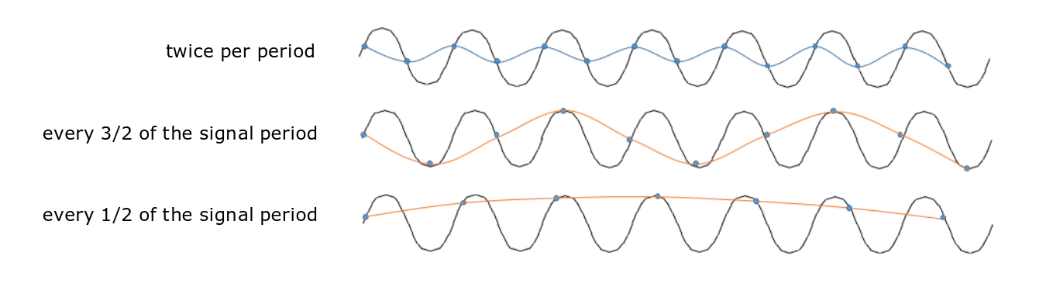
\includegraphics[width=0.7\textwidth]{Images/Pasted image 20251007085600.png}
    \caption{Aliasing example in a sine wave}
\end{figure}

\subsubsection{Quantization}
\begin{itemize}
    \item Digital values are finite: we cannot represent continuous values precisely!
    \item Quantization always introduces an error, which is the sensor's natural error.
    \item More bits, better resolution (but more data)
\end{itemize}

\begin{figure}[h]
    \centering
    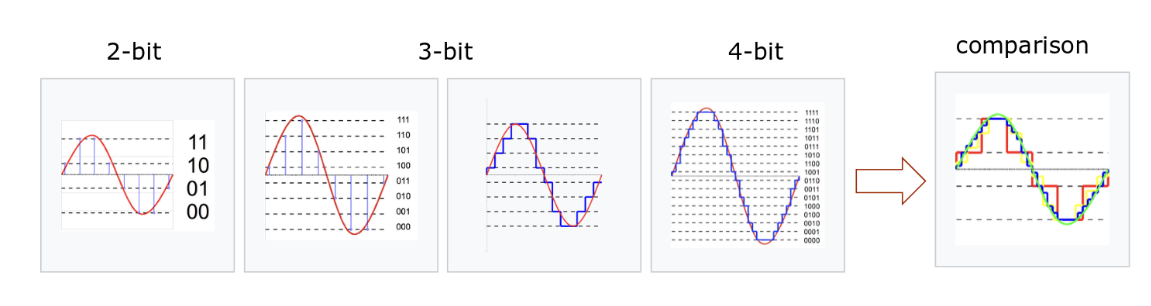
\includegraphics[width=0.7\textwidth]{Images/Pasted image 20251007085902.png}
    \caption{Quantization error illustration}
\end{figure}

\subsubsection{Saturation}
\begin{itemize}
    \item Sensors often have an upper limit, which is either physical or dictated by the maximum quantization level: in this case, we have saturation (all higher values are mapped to the same output)
    \item This is what happens when you take a picture with high exposure: all lighter points are bright white!
\end{itemize}

\begin{figure}[h]
    \centering
    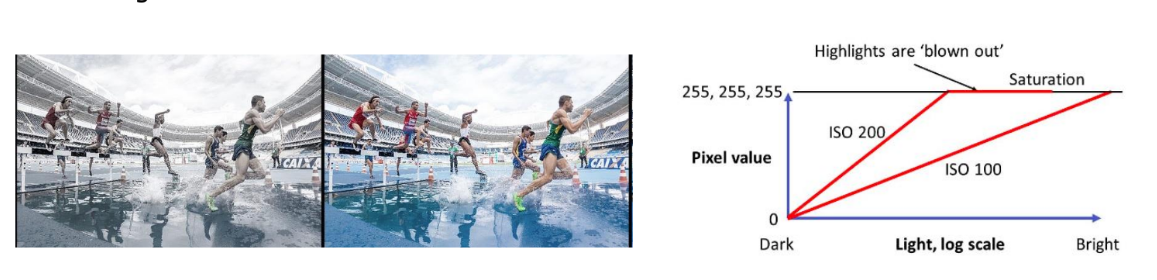
\includegraphics[width=0.7\textwidth]{Images/Pasted image 20251007090152.png}
    \caption{Saturation effect}
\end{figure}

\subsubsection{Hysteresis}
\begin{itemize}
    \item Sometimes sensors takes a while to track the process because the \textbf{physical nature of the measurement is slow}
    \item Which means we have Hysteresis error when the delay of sensor measurements depends on the magnitude of the change.
    
    \item Example: When you apply pressure to a sensor and then release that pressure, the sensor's output should in theory return you to the same value it started at before that specific pressure cycle. However, in reality, there are often small differences between the initial value and the final value after a pressure cycle.
    \begin{itemize}
        \item From 0 to 100 bar
        \item 0 bar $\rightarrow$ 0 V
        \item 100 bar $\rightarrow$ 2500 V
        \item 0 bar $\rightarrow$ 0.05 V
        \item \textbf{0.02\% / 1 bar hysteresis}
    \end{itemize}
\end{itemize}

\subsubsection{Non-linearities}
\begin{itemize}
    \item Ideally, sensors should also have linear responses: in reality, there are often non-linear effects that we need to adjust for.
    
    \item Hard to predict
    
    \item Example: A linear sensor's output will change by equal amounts for equal pressure changes across its entire range.
    \begin{itemize}
        \item From 0 to 10 bar
        \item 0 bar $\rightarrow$ 0 V
        \item 10 bar $\rightarrow$ 5 V
        \item 3 bar $\rightarrow$ 4.2 V (while I would have expected 3.75 V, according to the previous data).
        \item \textbf{$\leq$2\% non-linearity of full scale}
    \end{itemize}
\end{itemize}

\subsubsection{Calibration}

\begin{itemize}
    \item Sensors often require calibration to give proper results:
    \begin{itemize}
        \item Bias is a constant error term in one direction.
        \item Distortion is due to non-linearity.
    \end{itemize}
    
    \item By measuring a series of known quantities, we can compensate for these issues (however, external factors such as temperature can throw off calibration!)
    \item Example: Using the data from the calibration sheet, we see that the deviations are all less than the maximum deviation allowed of 0.5\%.
\end{itemize}

\subsubsection{Error propagation}
\begin{itemize}
    \item Calculations can change the error of a measurement, as the errors are also considered in the function you compute.
    \item Non-linear functions can have weird effects with measurement errors.
    \item Derivation (e.g., computing velocity from position measurements) is brittle: since the measurements are close together, noise can have a huge effect.
    \item Integration/averaging are robust (rely on many points, and noise is compensated).
    \item Example: Calculating heat index
    \begin{itemize}
        \item Temperature sensor: measured (30°) with uncertainty $\pm$0.5
        \item Humidity sensor: measured (70\%) with uncertainty $\pm$2\% (= 0.02)
        \item Heat index = T + 0.33$\times$RH$-$0.7 = 52.4
        \item \textbf{Uncertainty with error propagation: 0.828 $>$ (0.5 + 0.02)}
    \end{itemize}
\end{itemize}

\subsubsection{External data communication}
\begin{itemize}
    \item Sensors data may need to be shared with external parties, such as other peer nodes at the edge, fog, and cloud levels.
    \item Messages exchanged between IoT nodes may be delivered using \textbf{push} or \textbf{pull} modes.
    \begin{itemize}
        \item \textbf{Pull}: a message is explicitly requested from the source (server) by its recipient, an IoT client.
        \item \textbf{Push}: the data source and the gateway send data when the specified conditions are met, such as arrival of the data sampling time mark, or exceeding of the measurement threshold.
    \end{itemize}
    \item \textbf{Publish/subscribe system}: data sources ``publish'' data to a known place, and authorized clients can ``subscribe'' to data of interest and receive related messages.
    \begin{itemize}
        \item Publishers do not need to know the identity or number of their receivers (subscribers), and the receivers do not need to know the identity or state of their publishers.
    \end{itemize}
\end{itemize}

\paragraph{How to share sensors' data?}
\begin{itemize}
    \item Some processes (e.g., an electricity meter, a room thermostat) do not need to be sampled very often.
    \item If we only care about cumulative measures (how much electricity was consumed in total), we do not need frequent samples!
    \item On the other hand, faster processes need frequent samples, as process can change faster.
    \item Why don't we transmit all the time?
    \item There are several reasons why we cannot transmit all the time, but we will concentrate on two of them in this first part of the course:
    \begin{itemize}
        \item Limited bandwidth
        \item Limited energy
    \end{itemize}
    \item Each transmission (and, in fact, each activity the sensor performs) costs energy, as well as blocking the wireless channel for other transmissions
\end{itemize}

\paragraph{Some solutions to send sensors' data more efficiently}
\begin{itemize}
    \item \textbf{Interpolation}
    \begin{itemize}
        \item Interpolation is the mathematical tool to infer missing data from sparse samples. We have to make some assumptions on the nature of the process to be able to interpolate: if we have the correct model, we can send a lot fewer data samples!
        \item Interpolation can also be dangerous: we can underfit (select a model that is too simple) or overfit (select a model that is too complex and ends up following random noise).
    \end{itemize}
\end{itemize}

\begin{figure}[h]
    \centering
    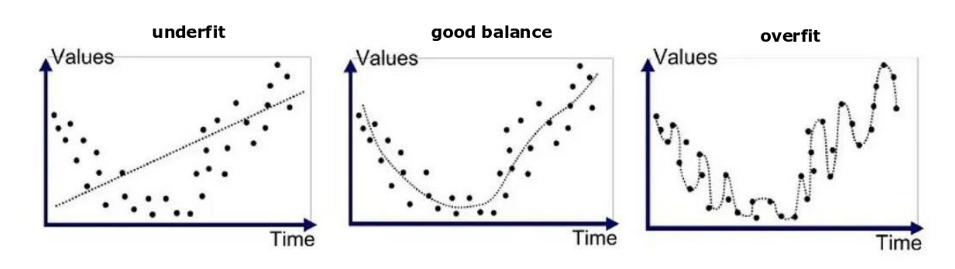
\includegraphics[width=0.7\textwidth]{Images/Pasted image 20251007093806.png}
    \caption{Interpolation: underfitting and overfitting}
\end{figure}

\begin{itemize}
    \item \textbf{Spatial correlation}
    \begin{itemize}
        \item Data are usually correlated in space:
        \begin{itemize}
            \item Traffic on either side of a bridge.
            \item Temperatures close together.
        \end{itemize}
        \item There can be easy natural relations (points close together are similar) or structural relations (connected points are similar).
        \item Since measurements have errors, correlations help us improving the quality of estimates: we can make statistical calculations and estimates to figure out what is happening in points (like the purple one on the bridge) where we have no sensors, or refine our estimates.
    \end{itemize}
    
    \item \textbf{Temporal correlation}
    \begin{itemize}
        \item Data are also correlated in time:
        \begin{itemize}
            \item Traffic in one spot
            \item Temperature measured by one sensor
        \end{itemize}
        \item The relation here can be more or less complex, and depend on space as well (e.g., line at a traffic light), but we can also exploit this to get better data with fewer transmissions.
        \item Correlations can be misleading and dangerous! When relying on statistical information to reconstruct missing data or make decisions, we need to be aware that random chance is always a possibility.
    \end{itemize}
\end{itemize}

\subsubsection{Local control}

\begin{itemize}
    \item Provided in systems where latency is critical and/or edge autonomy is required.
    \item Local control enables the edge node to execute pre-defined control sequences when a specified condition occurs on some combination of local data.
    \item If This Then That: scenes where lights and heating/cooling are adjusted accordingly when users are leaving or approaching their homes.
    \item \textbf{Node-RED}: provides a graphical user interface to construct data flows with the functional processing modules and actuation output stages.
    \item In the extreme case of temperature, the script triggers the device shutdown.
\end{itemize}

\begin{figure}[h]
    \centering
    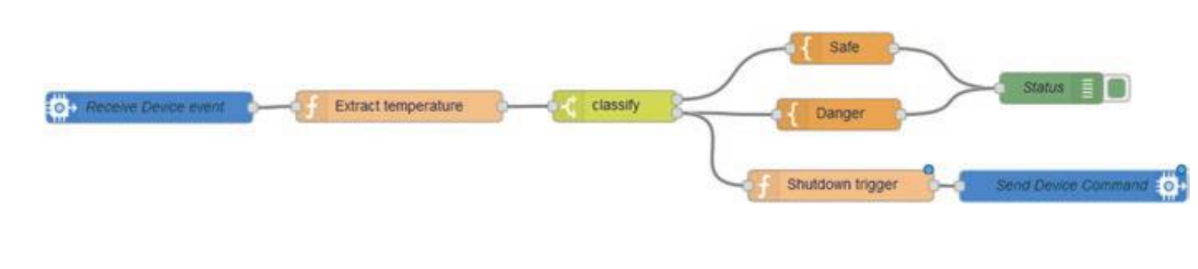
\includegraphics[width=0.8\textwidth]{Images/Pasted image 20251007094532.png}
    \caption{Node-RED example}
\end{figure}

\subsubsection{Data storage}
\begin{itemize}
    \item Data storage for the acquired data may be provided by the gateway.
    \item The existence of local storage provides the flexibility to conserve network bandwidth and to reduce the load on cloud resources by selectively reporting data that meet certain conditions.
    \begin{itemize}
        \item \textbf{Semantic communication.}
        \item Depending on the nature of the physical thing being measured, \textbf{only some of the data points may be of interest}. E.g., successive minor changes may be of little interest, but those that exceed a comfort guard band or change by a significant percentage or amount from prior readings are.
        \item Qualifying readings may be defined as events and reported only when they occur, with raw readings stored in the local database should they be required for auditing or subsequent analysis.
    \end{itemize}
\end{itemize}

\subsubsection{(Edge) analytics}
\begin{itemize}
    \item Edge analytics for the data may be provided by the gateway or the fog node.
    \item Proximity to data sources: low latency.
    \item Ability to process high-frequency data samples (at the rate of the sensor) $\rightarrow$ real-time.
    \item Conservation of network bandwidth by not sending data to the cloud.
    \item Can operate even in disconnected mode.
    \item Analytics generally require AI/ML models:
    \begin{itemize}
        \item Insufficient computational resources at the edge.
        \item No data aggregation of edge/local data.
    \end{itemize}
    \item IoT systems should be implemented using design tools and practices that facilitate flexible allocation of functions (in tandem between edge and cloud).
\end{itemize}

\subsubsection{Analytics placement}
\begin{itemize}
    \item Optimal placement of data and processing functions is an age-old trade-off in distributed systems.
    \item It is based on whether it is more cost-effective to move the data to the computation or to move the computation to the data, depending on:
    \begin{itemize}
        \item Availability and cost of bandwidth
        \item Latency requirements for time-critical operations
        \item Local autonomy of operations, including disconnected mode
        \item Security and data control or privacy concerns
        \item Cost and complexity of managing distributed nodes with computing and storage
        \item Available energy resources
        \item Available computational capacity
        \item \ldots
    \end{itemize}
\end{itemize}

\section{Control plane functions}
\begin{itemize}
    \item Fully functional gateways may be fairly sophisticated computational and communications nodes that host and execute a variety of services.
    \item They need to be properly secured and managed.
    \item Main control functionalities:
    \begin{itemize}
        \item Fault management (troubleshooting, error logging, and recovery).
        \item Remote monitoring, control, administration, and diagnostics.
        \item Remote firmware and software updates.
        \item Security updates.
        \item Metering (network bandwidth and software usage) and supervision.
        \item Provisioning and authentication.
    \end{itemize}
\end{itemize}

\subsection{(Cyber)security}

\begin{itemize}
    \item The first step is to determine the security risk.
    \item Identify, quantify, and prioritize the risks for the system, and find a balance between costs and potential losses from residual risks.
    \item Model to quantify risk: vulnerability, threats, and impacts.
\end{itemize}

\begin{figure}[h]
    \centering
    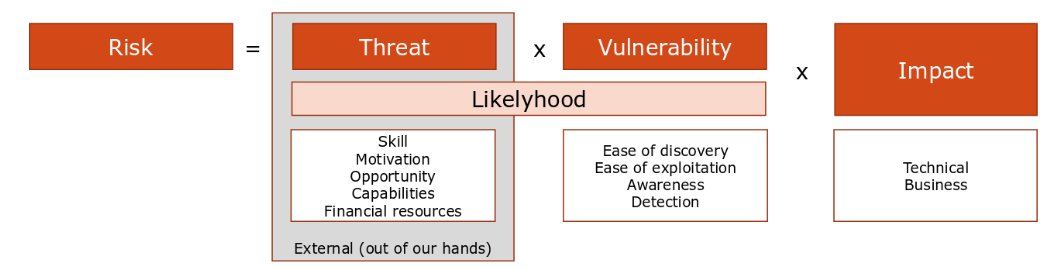
\includegraphics[width=0.6\textwidth]{Images/Pasted image 20251007095925.png}
    \caption{Security risk model}
\end{figure}

\begin{itemize}
    \item \textbf{Vulnerabilities}: can originate from the design of the system architecture, technology, and protocols, but more often emerge in the implementation (e.g., coding flaws) and in the operation phases (e.g., configuration errors, use of weak credential, unparched devices, unexpert use, etc.).
    
    \item \textbf{Security measures for the diligent user}:
    \begin{itemize}
        \item Partitioning the system into zones (characterized in terms of security levels).
        \item Adopt effective authentication protocols, tailored to the different zones.
        \item Provide cryptographic protection of data.
        \item Install equipment from trusted providers.
        \item Make and install frequent patches and workarounds (software updates).
        \item \ldots
    \end{itemize}
    
    \item \textbf{Threat}: an IoT network is a possible point of attack if the endpoint is unguarded and is positioned in an easily reachable position.
    \begin{itemize}
        \item \textbf{Eavesdropping}: learning confidential information.
        \item \textbf{Traffic analysis}: learning data origin, destination, and length (not the content).
        \item \textbf{Forgery}: building a fake message, pretending it was sent by someone else.
        \item \textbf{Masquerade}: claiming to be someone else in a single message.
        \item \textbf{Repudiation}: denying having sent or received a message.
        \item \textbf{Profiling}: gathering information about a single user.
        \item \textbf{Fingerprinting}: identifying the user associated with a message.
        \item \textbf{Jamming}: causing interference to a communication.
    \end{itemize}
    
    \item \textbf{Standards}: IoT-oriented and industry-specific standards have been developed for security.
\end{itemize}

\begin{figure}[h]
    \centering
    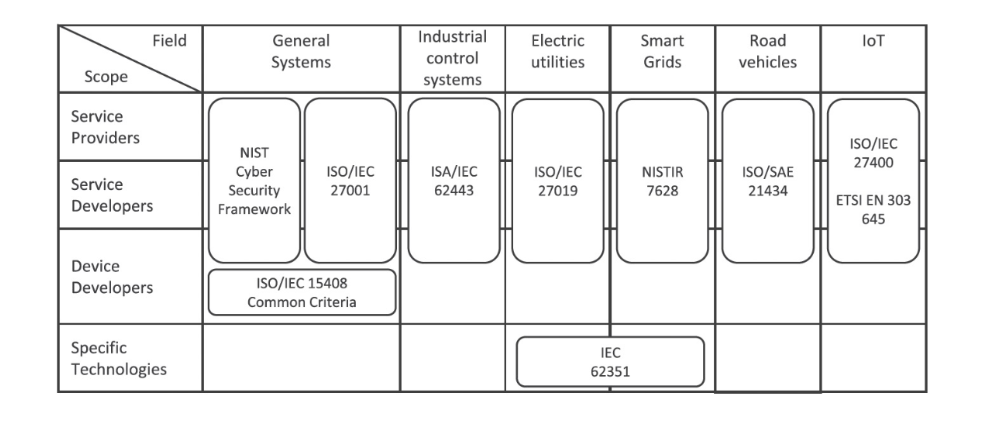
\includegraphics[width=0.7\textwidth]{Images/Pasted image 20251007100557.png}
    \caption{IoT security standards}
\end{figure}

\subsection{Provisioning and authentication}
\begin{itemize}
    \item \textbf{Provisioning}: the lifecycle of an endpoint begins with its provisioning in the network.
    \item It is the process of giving the endpoint the configuration data and the ability to present itself.
    \item \textbf{Authorization}: checking the rights of access to the network.
    \item \textbf{Application-level authentication}: used if the network is shared among applications.
    \item \textbf{Authentication}: verification of the identity (``I know your name, is it you?'').
    \item \textbf{Challenge-response protocol}: employs secret keys for verification.
\end{itemize}

\begin{figure}[h]
    \centering
    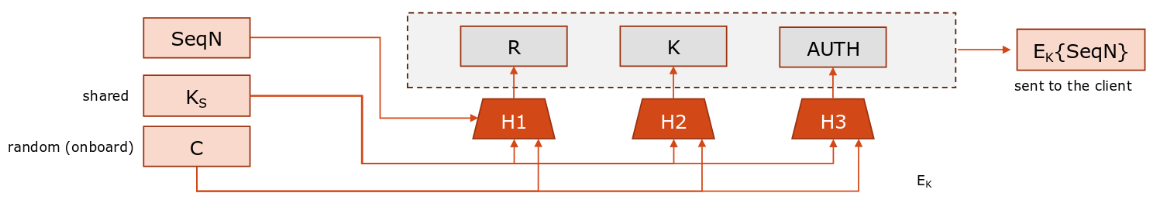
\includegraphics[width=0.6\textwidth]{Images/Pasted image 20251007101013.png}
    \caption{Challenge-response protocol}
\end{figure}

\section{QoS and performance}

\begin{itemize}
    \item \textbf{One-way delay (OWD)}: time between the transmission of the first bit of a packet at an interface and the reception of the last bit of the packet at the other interface.
    \item Requires perfect time synchronization between the endpoints.
    \item \textbf{Time reference}: Network Time Protocol (NTP).
    \item \textbf{Two-way delay (TWD)}: time between the transmission of the first bit of a packet at an interface and the reception of the last bit of the packet at the same interface, after being reflected by the system at the other end, net of the End System Delay (ESD, processing time at the remote node).
    \item We have that \textbf{Round Trip Time (RTT) = TWD + ESD.}
\end{itemize}

\subsection{Delay}
\begin{itemize}
    \item \textbf{Packet-delay variation (PDV)} ($\sim$jitter): based on previous OWD/TWD measures.
    \begin{itemize}
        \item PDV = $|$OWD$_i$ - OWD$_{i-1}|$
        \item PDV = $|$OWD$_i$ - mean\{OWD\}$|$
        \item PDV = $|$OWD$_i$ - min\{OWD\}$|$
        \item PDV = $|$OWD$_i$ - OWD$_1|$
        \item \ldots
    \end{itemize}
    
    \item \textbf{Problem}: These delay metrics do not consider the MAC delay (for channel access).
    \item \textbf{End-to-end delay (E2E)}: it consists of (at least) three components:
    \begin{itemize}
        \item \textbf{MAC delay} (under the control of the system designer).
        \item \textbf{Access link and gateway delay} (under the control of the system designer).
        \item \textbf{OWD} (depends on the WAN).
    \end{itemize}
\end{itemize}

\subsubsection{Delay and ``real-time''}
\begin{itemize}
    \item The expression \textbf{``real-time''} may have different interpretations:
    \begin{itemize}
        \item \textbf{Synchronization} to a common time reference.
        \item \textbf{Responding fast.}
        \item \textbf{Responding within predictable response times.}
    \end{itemize}
    
    \item \textbf{Hard real-time}: if the response exceeds a limit, the system does not operate well.
    \begin{itemize}
        \item Example: respond within 5 ms
        \item \textbf{CASE 1:} The application always responds in 4 ms
        \begin{itemize}
            \item Average delay: 4 ms; Failure rate: 0\%
        \end{itemize}
        \item \textbf{CASE 2:} The application responds in 1 ms for 99.9\% of the times, and in 6 ms in 0.01\%.
        \begin{itemize}
            \item Average delay: 1.005 ms; Failure rate: $10^{-3}$
        \end{itemize}
    \end{itemize}
    \item \textbf{Soft real-time}: it involves some response time percentiles.
\end{itemize}

\subsection{Packet loss}
\begin{itemize}
    \item In an IoT network, \textbf{loss may occur} if:
    \begin{itemize}
        \item The \textbf{buffers of a node overflow.}
        \item \textbf{Transmission errors} (negligible in wired LANs, dominant in wireless LANs).
        \item \textbf{Delay much larger than expected} may be considered as a loss.
    \end{itemize}
    
    \item How to have realistic measures of packet loss? There are some problems:
    \begin{itemize}
        \item \textbf{Long-lasting measurements:} averaging of data gives no indications on the short period.
        \item \textbf{Short measurements:} no statistically meaningful data.
        \item \textbf{Intense bursts:} too intrusive, altering the result (not representative of a real situation).
    \end{itemize}
\end{itemize}

\subsection{Capacity}
\begin{itemize}
    \item \textbf{Hardly a problem}, as applications are not (in general) bandwidth demanding.
    \item For some high-end applications (e.g., telemedicine, IIoT, automotive, etc.), \textbf{capacity} is generally less important than other metrics such as reliability.
    \item \textbf{Example:} metering application
    \begin{itemize}
        \item Collect 1M samples (or sensors?) (of 128B) every 15 minutes.
        \item \textbf{Average throughput:} 1,000,000 $\times$ 128B $\times$ 8 (bit) / (15 $\times$ 60) = 1.3 Mbit/s
        \item If the same measurements take place as unsolicited events from the endpoint in the same second, the \textbf{link capacity} shall be around 1,000,000 $\times$ 128B $\times$ 8 (bit) = 1 Gbit/s.
    \end{itemize}
\end{itemize}

Those are the most important metrics, but there are other ones related to IoT.

\subsection{Reliability}
\begin{itemize}
    \item \textbf{R(t)}: probability that a system is working as expected at a certain time \textit{t.}
    \begin{itemize}
        \item For most systems, the early phase of ``high mortality'' is short and occurs during tests.
        \item The system is generally replaced for obsolescence as the aging phase approaches.
        \item In ``normal life'', most systems shall be reliable.
    \end{itemize}
    \item \textbf{R(t)} is memoryless: the residual life of failure does not depend on how long the system has been working $\rightarrow$ the system does not age during ``normal life.''
\end{itemize}

\begin{figure}[h]
    \centering
    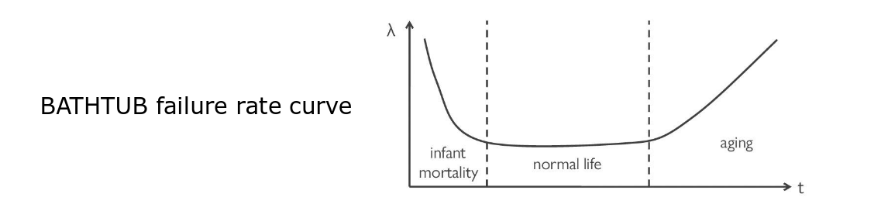
\includegraphics[width=0.6\textwidth]{Images/Pasted image 20251008085321.png}
    \caption{Reliability curve}
\end{figure}

\subsection{Availability}
\begin{itemize}
    \item \textbf{Probability that the system is working} when observed at a random time instant.
    \item We assume that the system can be periodically repaired if needed and put back in service.
    \item \textbf{Mean Time Between Failures (MTBF).}
    \item \textbf{Mean Time To Repair (MTTR).}
\end{itemize}

$$
A = \frac{MTBF}{MTBF + MTBR}
$$

\begin{figure}[h]
    \centering
    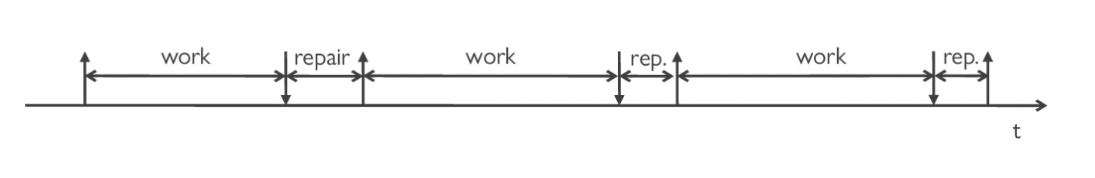
\includegraphics[width=0.6\textwidth]{Images/Pasted image 20251008085509.png}
    \caption{Availability illustration}
\end{figure}

\subsubsection{Availability (example)}
\begin{itemize}
    \item For memoryless systems, \textbf{MTBF = Mean Time To Fail (MTTF) = 1/$\lambda$.}
    
    \item \textbf{Example:} prevention of fires in a forest
    \begin{itemize}
        \item \textit{N} sensors that monitor fires in the forest.
        \item Sensors fail at rate \textbf{$\lambda$.}
        \item The prevention works if \textit{x\%} of sensors are active and alive.
        \item Period of effectiveness of the system (\textbf{T}):
    \end{itemize}
\end{itemize}

$$
N e^{-\lambda T} = xN \quad \Rightarrow \quad T = \frac{-\ln x}{\lambda}
$$

\section{Energy constraints}

\subsection{Introduction}

\begin{itemize}
    \item Most sensors and components use electrical energy, i.e., they exploit the movements of electrons across a conducting medium.
    \item Powering is a very important issue, and depends on the endpoint capabilities and the network architecture procedures.
\end{itemize}

\begin{table}[h]
\centering
\begin{tabular}{|l|l|}
\hline
\textbf{Type} & \textbf{Examples} \\
\hline
\textbf{Mains / manually recharged} & Field buses Smartphones Smart grid devices \\
\hline
\textbf{Battery} & Most sensors \\
\hline
\textbf{Data line} & Videocameras \\
\hline
\textbf{Harvesting} & Environmental sensors \\
\hline
\end{tabular}
\caption{Energy sources for IoT devices}
\end{table}

\subsection{Sources of consumption}

\subsubsection{Computing}

\begin{itemize}
    \item Computing requires a certain energy for each cycle, corresponding to one basic operation. Some operations (e.g., sinusoidal functions) require multiple cycles.
    \begin{itemize}
        \item Energy consumption is usually a function of the number of cycles required.
    \end{itemize}
    \item If a device has a certain clock frequency, we can also compute the power it requires to perform calculations.
    \item Computing energy can be formalized based on the number of logical operations that are required to perform: \textbf{AND, NOT, OR, XOR.}
\end{itemize}

\subsubsection{Boards and PLCs}
\begin{itemize}
    \item Boards and PLCs are standard circuits used in industrial automation. Larger IoT nodes also use Arduinos or other pre-made boards.
    \item Smaller, more efficient nodes are often designed ad hoc, to use as little energy as possible. In general, IoT nodes have limited computational capabilities.
\end{itemize}

\textbf{Example: Arduino-UNO}

The Arduino Uno is a microcontroller board based on the ATmega328.
It contains everything needed to support the microcontroller; simply connect it to a computer with a USB cable or power it with an AC-to-DC adapter or battery to get started.

\subsubsection{Communication}

\begin{itemize}
    \item Digital communication usually requires more steps than just sending a wave, and each consumes energy:
    \begin{enumerate}
        \item \textbf{Encoding and error protection.}
        \begin{itemize}
            \item Use known redundant codes: the simplest example is the parity check bit.
            \item Decoders are often complex, but can correct errors in transmission and recover the original packet. However, complexity is paid for in energy.
        \end{itemize}
        
        \item \textbf{Preambles for synchronization and channel estimation.}
        \item \textbf{Modulation} from the baseband digital signal to the passband analog signal.
        \item \textbf{Transmission} (power is applied to the antenna) (not required for reception).
        \begin{itemize}
            \item IoT transmissions are usually slow (low bitrate), but distance plays a large role.
        \end{itemize}
    \end{enumerate}
\end{itemize}

\subsection{Source of energy}

\subsubsection{Mains power}
\begin{itemize}
    \item Provide virtually unlimited power, making it possible to employ complex protocols, work at high bitrates, and achieve long-distance communication.
    \item There are some drawbacks:
    \begin{itemize}
        \item Only work in wired fixed systems.
        \item Can be dangerous in environments at risk of fire and explosions.
        \item Need to lay out an electric line (challenging in hard-to-reach remote/rural areas).
        \item Need to put transformers (expensive).
    \end{itemize}
\end{itemize}

\subsubsection{Power over Ethernet (PoE)}
\begin{itemize}
    \item Employ the wired communication infrastructure also for powering.
    \item Can carry DC power on the twisted pair used for Ethernet connectivity.
    \item Only one cabled infrastructure needs to be in place.
    \item Transformers are not needed.
\end{itemize}

\subsubsection{Powerline communication}
\begin{itemize}
    \item It is the opposite of PoE.
    \item Use the powerline to carry data.
    \item Based on modulation between high-frequency data and low-frequency electricity.
    \item Only one cabled infrastructure needs to be in place.
    \item Advantageous when the system to be monitored and controlled is the power grid itself.
\end{itemize}

\begin{figure}[h]
    \centering
    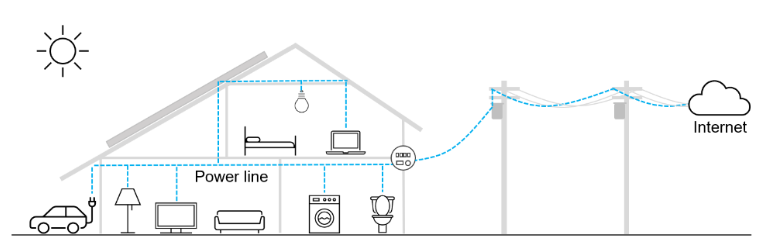
\includegraphics[width=0.7\textwidth]{Images/Pasted image 20251008091052.png}
    \caption{Powerline communication}
\end{figure}

\subsubsection{Batteries}
\begin{itemize}
    \item Batteries use the charge difference between ions to induce a potential difference.
    \begin{itemize}
        \item \textbf{Rechargeable} batteries can run the circuit backwards and move the electrons back (by connecting a stronger generator).
        \item Charging is never perfect: chemical impurities build up.
    \end{itemize}
    \item If the battery runs out completely, it is often impossible to recharge without direct intervention (which may be expensive): the objective is \textbf{never to let it run out!}
    \begin{itemize}
        \item Apply \textbf{statistical data} and direct information from the meter to define a plan of \textbf{proactive} on-field \textbf{intervention} if needed $\rightarrow$ carry out with proper timing to minimize the number of substitutions in the lifetime and the number of dedicated ``truck rolls'' or manual readings.
    \end{itemize}
\end{itemize}

\subsubsection{Batteries (management and optimization)}
\begin{itemize}
    \item Energy is the basic constraint of IoT systems. What can we do?
    \begin{itemize}
        \item Employ battery technology with low self-discharging properties.
        \item Minimize the duration of active states of the radio components with suitable scheduling algorithms and MAC protocols.
        \begin{itemize}
            \item Duty cycles, sleep mode, alert/notification, etc.
        \end{itemize}
        \item Adopt energy-aware routing.
        \item Introduce endpoint management protocols that communicate the state of batteries.
        \item Adopt a ``let it be off'' approach.
        \item Recharge batteries with energy harvesting.
    \end{itemize}
\end{itemize}

\subsubsection{Energy harvesting}
\begin{itemize}
    \item Energy harvesting: recharge it while it is running.
    \item Energy harvesting sensors and actuators are equipped with some kind of generator and can recharge their battery from it. This allows them to stay alive much longer than with a single battery charge, even if they get very little energy.
\end{itemize}

\begin{figure}[h]
    \centering
    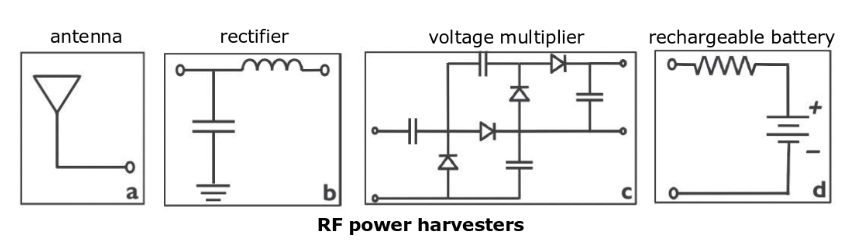
\includegraphics[width=0.7\textwidth]{Images/Pasted image 20251008091530.png}
    \caption{Energy harvesting methods}
\end{figure}

\subsubsection{Solar and wind energy}
\begin{itemize}
    \item \textbf{Solar panels} are now cheap, and solar energy is renewable and clean.
    \begin{itemize}
        \item The sensor needs to be exposed (shade can be a problem, underground or indoor sensors will not work).
        \item Photovoltaic cells will not generate any power at night (the sensor needs to get through the night on a single charge).
    \end{itemize}
    \item Another possibility is wind energy, but there are several challenges:
    \begin{itemize}
        \item The sensor still needs to be exposed (underground or indoor sensors will not work).
        \item Wind is intermittent and unpredictable.
        \item Small turbines are inefficient.
    \end{itemize}
\end{itemize}

\subsubsection{Thermal and vibration energy}
\begin{itemize}
    \item \textbf{Thermal energy} is cheap when the sensor has access to temperature gradients:
    \begin{itemize}
        \item The inside/outside or ground/air gradient can generate energy.
        \item The power is usually very small, but may be the only option for buried sensors.
        \item Need for long distances between terminals.
        \item Good for wearables: the difference between body temperature and the air is high.
    \end{itemize}
    \item Vibration energy can be collected using piezoelectric devices with good efficiency.
    \item The constant presence of vibrations energetic enough to power the endpoint is uncertain, except in some industrial environments.
\end{itemize}

\subsubsection{Wireless power transfer (WPT)}
\begin{itemize}
    \item Sensors can benefit from the power of received transmissions, but the benefits are tiny at longer distances: this is only feasible for very low-power sensors.
    \item \textbf{Inductive coupling}: uses electromagnetic fields to transfer energy between coils.
    \item \textbf{Capacitive coupling}: transfers energy via electric fields between conductive plates.
    \item Uses \textbf{RF signals} to transfer power over longer distances (several meters to kilometers).
    \item Uses \textbf{focused laser beams} to transmit power over long distances.
\end{itemize}

\subsubsection{Passive sensors}
\begin{itemize}
    \item We can also use the received transmission to power the circuit directly: \textbf{RFID tags, biometric passports, and contactless cards} work this way.
    \item Power loss is huge: these only work over short distances.
    \item The sensor cannot actively transmit or record data, only respond to messages.
    \item There are \textbf{privacy issues} (anyone can read a tag, the only limit is the SNR).
\end{itemize}

\begin{figure}[h]
    \centering
    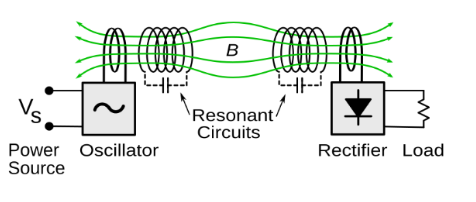
\includegraphics[width=0.6\textwidth]{Images/Pasted image 20251008091951.png}
    \caption{Passive sensors (RFID)}
\end{figure}
